\chapter{Manual del juego en 3D}

\section{Estructura de las escenas}

La estructura del videojuego es la siguiente: 

\begin{figure}[H]
	\centering
	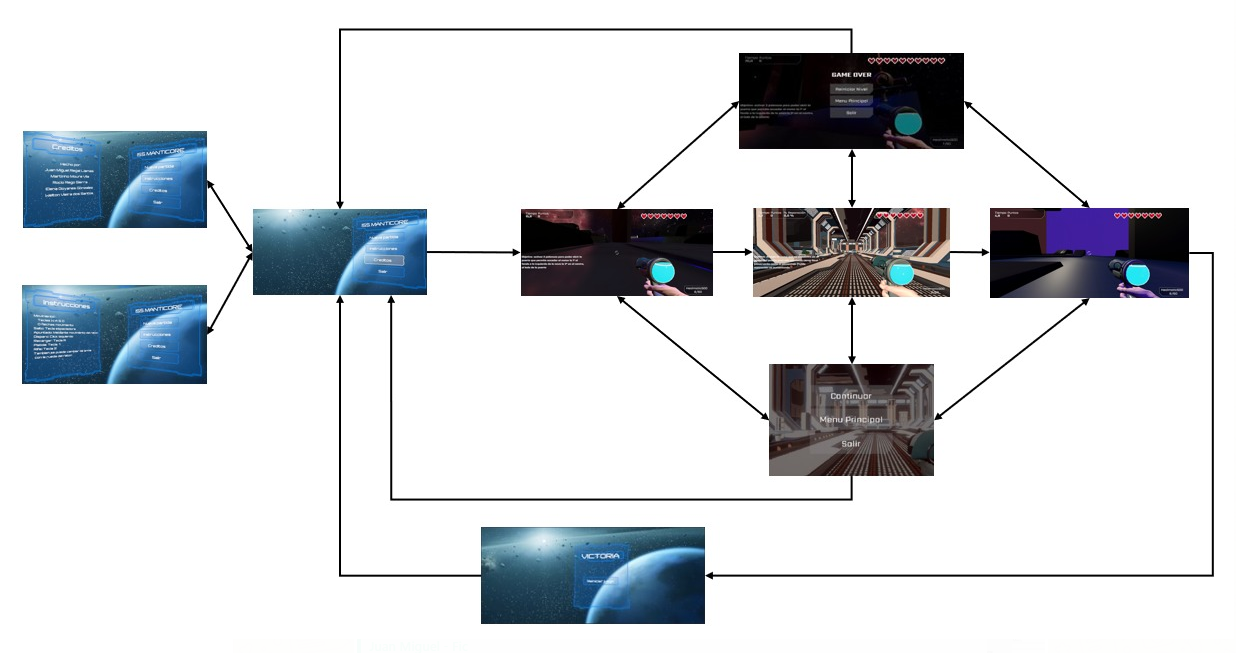
\includegraphics[scale=0.50]{imagenes/estructuraEscena3D.png}
	\caption{\label{fig:EstructuraEscena3D}Estructura de las escenas del video juego}
\end{figure}

\section{Controles}

Las teclas WASD y las flechas del teclado permiten que el jugador se mueva por el escenario en las direcciones de las flechas. Para manejar la cámara, es decir, lo que ve el personaje se utiliza el ratón para ese cometido. Figura \ref{fig:flechasTeclado}.

\begin{figure}[H]
	\centering
	\includegraphics[scale=0.40]{imagenes/teclasWASD.png}
	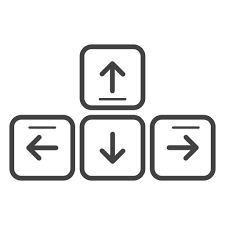
\includegraphics[scale=0.50]{imagenes/flechas_teclado.png}
	\caption{\label{fig:flechasTeclado}Teclas de movimiento del personaje}
\end{figure}

El ratón permite que el jugador apunte y dispare los proyectiles a sus enemigos con el click izquierdo.

\begin{figure}[H]
	\centering
	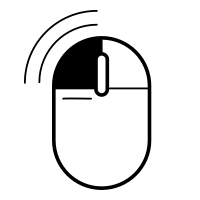
\includegraphics[scale=0.50]{imagenes/raton.png}
	\caption{\label{fig:raton}Raton y click izquierdo}
\end{figure}

La tecla escape permite al jugador acceder al menú de pausa
\begin{figure}[H]
	\centering
	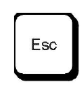
\includegraphics[scale=0.50]{imagenes/escape.png}
	\caption{\label{fig:escape}Tecla escape}
\end{figure}

Para efectuar un salto con el personaje se utiliza la tecla espacio del teclado.

Para efectuar el cambio del arma del personaje se utilizan las teclas 1 y 2 del teclado o haciendo un giro de la rueda del ratón.

\section{Ejecución del juego}
Para abrir el juego basta con ejecutar ``ISS\_Manticore.exe''.

\section{Navegación del Menú Principal}
Al iniciarse el juego aparece el menú de inicio con las siguientes opciones: 

\begin{figure}[H]
	\centering
	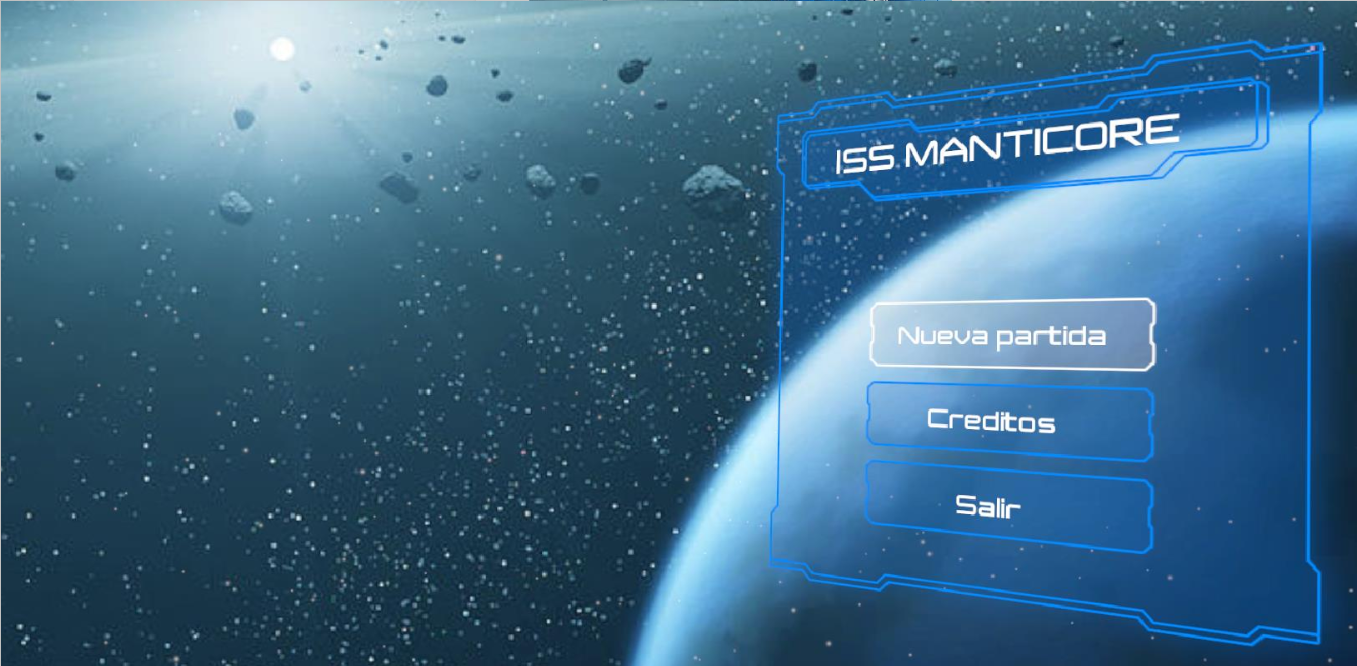
\includegraphics[scale=0.40]{imagenes/MenuPrincipal3D1.png}
	\caption{\label{fig:EjemploMenuPrincipal3D}Ejemplo del menú principal}
\end{figure}

Para desplazarse entre las distintas opciones se utilizan las flechas o las teclas WASD del teclado o el ratón.

Para seleccionar la opción deseada basta pulsar la tecla enter del teclado o efectuar un click con el botón izquierdo del ratón.

A continuación, se detallan cada una de ellas: 
\begin{itemize}
	\item \textbf{Nueva Partida:} Activa una segunda ventana en el menú con una explicación de los controles del juego  y un botón ``Continuar al juego'' (Figura \ref{fig:MenuPrincipalNuevaPartida}) que lleva al nivel 1.	
	\item \textbf{Créditos:} muestra la lista de nombres de los desarrolladores y del product owner (Figura \ref{fig:MenuPrincipalCreditos}).  
	\item \textbf{Salir:} cierra la ventana del juego. 
\end{itemize}



Tanto desde la pantalla de la leyenda como desde los créditos se puede retroceder al menú pulsando la tecla Esc. 


Cuando da comienzo la historia van apareciendo los diferentes niveles que el jugador debe superar, si este llega al final aparecerá un indicativo demostrando que ha finalizado el juego. Si por el contrario el jugador pierde todas sus vidas por el camino aparecerá otro indicativo manifestando la derrota. Tras terminar el juego, tanto con éxito como si no, es necesario pulsar la tecla Esc para volver al menú principal.    